\documentclass[12pt]{article}
\usepackage{amsmath}
\usepackage{amsfonts}
\usepackage{amssymb}
\usepackage{setspace}
\usepackage{mathtools}
\usepackage{graphicx}
\usepackage{tabularx}
\usepackage{hyperref}
\graphicspath{ {figures/} }
\usepackage{tikz}
\usepackage[margin=0.7in]{geometry}
\usepackage{fancyhdr}
	%\thispagestyle{fancy}
	
 \begin{document}

\newenvironment{myspace}[1]
	{\begin{spacing}{#1}}
	{\end{spacing}}

%----------------------------------------------------------------------------------------
%	TITLE PAGE
%----------------------------------------------------------------------------------------

\begin{titlepage} % Suppresses displaying the page number on the title page and the subsequent page counts as page 1
	\newcommand{\HRule}{\rule{\linewidth}{0.5mm}} % Defines a new command for horizontal lines, change thickness here
	
	\center % Centre everything on the page
	
	%------------------------------------------------
	%	Headings
	%------------------------------------------------
	
	\textsc{\LARGE Illinois Institute of Technology}\\[1.5cm] % Main heading such as the name of your university/college
	
	\textsc{\Large CS 425}\\[0.5cm] % Major heading such as course name
	
	\textsc{\large Database Organization}\\[0.5cm] % Minor heading such as course title
	
	%------------------------------------------------
	%	Title
	%------------------------------------------------
	
	\HRule\\[0.4cm]
	
	{\huge\bfseries CS425 Project: Online Distribution Center}\\[0.4cm] % Title of your document
	
	\HRule\\[1.5cm]
	
	%------------------------------------------------
	%	Author(s)
	%------------------------------------------------
	
	\begin{minipage}{0.4\textwidth}
		\begin{flushleft}
			\large
			\textit{Authors}\\
			Hector \textsc{Hernandez}\\
			Ramir \textsc{Aguilos}\\
			Rafael \textsc{Zavala}\\
			Hauyu \textsc{Wang}\\
		\end{flushleft}
	\end{minipage}
	~
	\begin{minipage}{0.4\textwidth}
		\begin{flushright}
			\large
			\textit{Professor}\\
			Dr. Omar \textsc{Aldawud} % Supervisor's name
		\end{flushright}
	\end{minipage}
	
	% If you don't want a supervisor, uncomment the two lines below and comment the code above
	%{\large\textit{Author}}\\
	%John \textsc{Smith} % Your name
	
	%------------------------------------------------
	%	Date
	%------------------------------------------------
	
	\vfill\vfill\vfill % Position the date 3/4 down the remaining page
	
	{\large February 28, 2018} % Date, change the \today to a set date if you want to be precise
	
	%------------------------------------------------
	%	Logo
	%------------------------------------------------
	
	%\vfill\vfill
	%\includegraphics[width=0.2\textwidth]{placeholder.jpg}\\[1cm] % Include a department/university logo - this will require the graphicx package
	 
	%----------------------------------------------------------------------------------------
	
	\vfill % Push the date up 1/4 of the remaining page
	
\end{titlepage}




\begin{myspace}{1.7}
        
\section*{Introduction}  
	This project consist of a web solution for an e-commerce web application regarding product distribution. From the web application, customers will have access to querying products from different suppliers. Employees of the web application will have specific views tailored to their tasks. The project itself will be conducted using a waterfall model \cite {waterfall} for development.
	The waterfall model consists of these ordered steps: Requirements, Design, Implementation, Verification, and Maintenance.
	The requirements that are set out for the development of a software project are constraints, usages, views, functions, and any other interaction between users and the software's interface. For this project, the requirements are listed as a list of functionalities that different users have with the product distribution system.
	The design of a software project is the development of blueprints or plans for how the development will be implemented. Design also consists of determining what medium and environment the project will be developed in. For the purposes of this project, the design consists of using Github repository as a functioning interaction between the project developers to create files necessary for the database driven software.
	The implementation of a software project will be the actual creation of the design plans. The implementation of the project will be a web-based application using a DBMS (database management software) as the back-end of the system and HTML, CSS, and PHP, with NodeJS as the front-end of the application.
	The verification of a software project is the running of tests to determine its readiness to be deployed as a product or service. For this project, testing will be driven by the methods of unit testing each aspect of the web application and having test users use the application.
	The maintenance of a web application occurs after a software project has been launched or deployed. Ideally, the maintenance of a web application occurs autonomously as the database and server structure will be able to maintain a state of software homeostasis where users can manage their access to the service without losing the integrity of data stored in the database. When there are cases such as data integrity loss or concurrency issues, the physical maintenance and restructuring software are necessary, which would require project developers to address. For this project, maintenance of the web application can be accomplished through many methods such as having more than one physical drive to store user data or creating 'watchdog' programs to monitor the state and integrity of the databases that do not rely on the main server.
	

%*********************************************************************************************
%*********************************************************************************************
%
%					Introduction
%
%*********************************************************************************************
%*********************************************************************************************
\pagebreak
\section*{Requirements}  

%*********************************************************************************************
%*********************************************************************************************
%
%				       Requirements
%
%*********************************************************************************************
%*********************************************************************************************

\begin{table}[]
\centering
\label{my-label}
\begin{tabular}{| p{.5cm}|p{9cm} |p{5cm}|}
\#  & Requirement Description                                                                                                                                                                                                                                                                                & Testing Criteria                                                                                                                                                                                                                                                               \\
R1  & The application shall allow customers to register with the application. The application shall present the user with a registration form with the following fields: Customer Name, Contact Name, Email, phone, region, address, major product line category (research a list that fits most customers). & User enters registration information and the data is stored in the Customer database.                                                                                                                                                                                        \\
R2  & Once a customer registers with the application the application shall generate a unique customer id.                                                                                                                                                                                                    & A unique customer is stored in the database.                                                                                                                                                                                                                                 \\
R3  & The system shall allow the customer to enter a password for her account. The password shall at least be 8 characters long and shall have at least one distinctive character and one uppercase character and a mixed alphanumeric value.                                                                & Customers password shall be encrypted and stored in the database.                                                                                                                                                                                                            \\
R4  & The customer shall be able be able to visit his/her profile within the application and be able to update his/her profile information only.                                                                                                                                                             & Customers information in the database is updated according to user input.                                                                                                                                                                                                    \\
R5  & The customer shall be able to query products online. with the following attributes: Name, Description, Categories, Units, Price.                                                                                                                                                                       & User enters product information and the application shows a list of relevant products.                                                                                                                                                                                       \\
R6  & The application shall allow the Supplier to register with the application. The application shall present the user with a registration form with the following fields: name, email, phone number, and address.                                                                                          & Supplier enters registration information and the data is stored in the Supplier database.                                                                                                                                                                                    \\
R7  & Once the supplier registers their product with the application, the application shall generate a unique product id and will also update the Categories database to include any new categories created or increase the relevance of any categories that exist already.                                  & 足      A unqiue product is stored in the Products database and the product is visible to any any customer within the application. Categories Database is updated accordingly based on how products are loaded onto the application.                                          \\
R8  & The customer should be able to add/remove products to their cart. Even when the user logs out, the cart is saved with all products from the previous session(s).                                                                                                                                       & Cart database, corresponding to the customer, is updated accordingly. Cart keeps products from the previous session until checkout or explicitly removed by the user. Cart displays price, quantity, title, and image of each desired product. Cart displays total expenses. \\
R9  & The customer shall have the option (button) to remove all products from the cart in one instance.                                                                                                                                                                                                      & A pop-up window confirms the deletion of all products in cart, then cart is emptied entirely.                                                                                                                                                                                \\
\end{tabular}
\end{table}
%*********************************************************************************************
%*********************************************************************************************
%
%				       Requirements
%
%*********************************************************************************************
%*********************************************************************************************

\begin{table}[]
\centering
\label{my-label}
\begin{tabular}{| p{.5cm}|p{9cm} |p{5cm}|}
\#  & Requirement Description                                                                                                                                                                                                                                                                                & Testing Criteria                                                                                                                                                                                                                                                               \\
R10 & The customer shall have the option to checkout with paypal or credit/debit card.                                                                                                                                                                                                                       & The application verifies the transaction. Once the transaction is verified, an e-mail confirmation of their placed ordered is sent to the customer. An e-mail confirmation is sent to the seller.                                                                            \\
R11 & Customer gets asked if he/she wants to save their payment information for future orders.                                                                                                                                                                                                               & Pop-up window confirms if the user wants to save payment information; if yes, payment information is stored.                                                                                                                                                                 \\
R12 & The customer shall be able to monitor the status of their order.                                                                                                                                                                                                                                       & The application allows the customer to view orders placed; the application                                                                                                                                                                                                   \\
R13 & The customer shall be able to search for products explicitly using a search engine within the application.                                                                                                                                                                                             & The application searches the Categories or Products databases to display items.                                                                                                                                                                                              \\
R14 & The customer shall be able to view their order history.                                                                                                                                                                                                                                                & The application provides a list of all orders made by the customer and the status and time stamp of each order.                                                                                                                                                              \\
R15 & The application shall display the status of each product.                                                                                                                                                                                                                                              & The application searches through the Product Database and assigns the status (In stock, Out of Stock, etc...) to the product based on quantity.                                                                                                                              \\
R16 & The application shall allow registered customers to sign-in via a sign-in page.                                                                                                                                                                                                                        & The sign-in page searches through the customer database to authenticate the user.                                                                                                                                                                                            \\
R17 & The application shall automatically display the most popular categories on the home page.                                                                                                                                                                                                              & The application should keep track of what categories and products are frequently searched for.                                                                                                                                                                               \\
R18 & The application shall allow warehouse managers to register with the application. The application shall present the warehouse manager with a registration form with the following attributes: Name, address, warehouse\_id, special password (provided by the company).                                 & The data is stored in the warehouse database and a unique manager id created.                                                                                                                                                                                                \\
\end{tabular}
\end{table}

%*********************************************************************************************
%*********************************************************************************************
%
%				       Requirements
%
%*********************************************************************************************
%*********************************************************************************************

\begin{table}[]
\centering
\label{my-label}
\begin{tabular}{| p{.5cm}|p{9cm} |p{5cm}|}
\#  & Requirement Description                                                                                                                                                                                                                                                                                & Testing Criteria                                                                                                                                                                                                                                                               \\
R19 & Warehouse managers can view customers in their region.                                                                                                                                                                                                                                                 & The application shall allow warehouse managers to view a list of customers (Name, address, region, and e-mail) in his/her region only.                                                                                                                                       \\
R20 & The application shall allow warehouse managers to view the inventory in their warehouse.                                                                                                                                                                                                               & The application should provide a list of all products that are in their respective warehouse.                                                                                                                                                                                \\
R21 & The application shall emphasize to the warehouse manager which products need to be prioritized for shipping.                                                                                                                                                                                           & By checking the time stamps of the orders or shipping service used, the application will output a filtered list of products.                                                                                                                                                 \\
R22 & Administrators have the priviledges of modyifing warehouses, product, employee, invoices, and customer data.                                                                                                                                                                                           & Administrator account(s) with these priviledges will be created.                                                                                                                                                                                                            
\end{tabular}
\end{table}

%*********************************************************************************************
%*********************************************************************************************
%
%				       Design
%
%*********************************************************************************************
%*********************************************************************************************
\pagebreak
\section*{Design}
\subsection*{Entity Relationship Diagram}
\begin{center}
          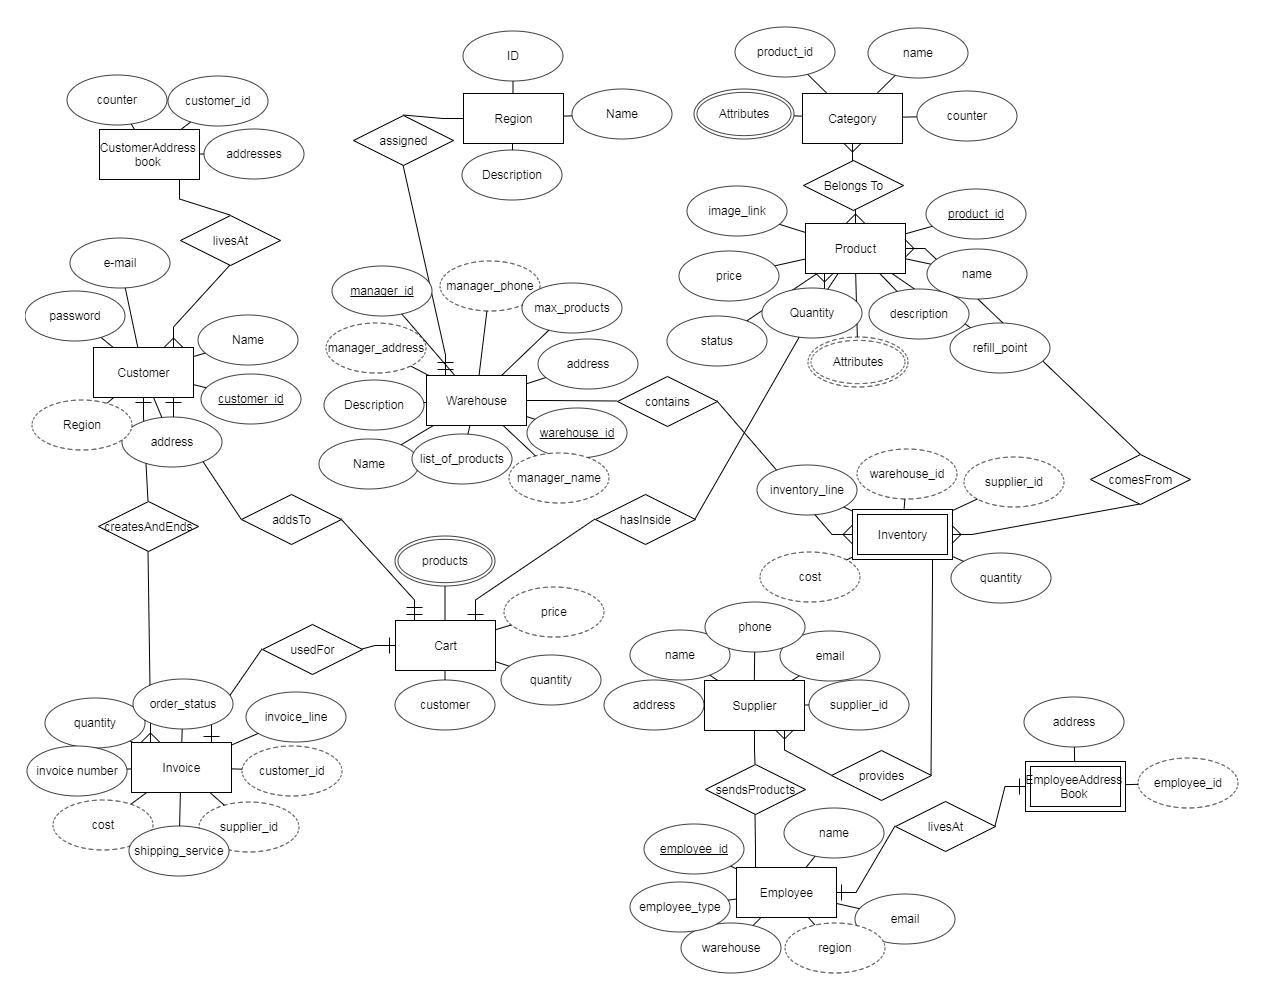
\includegraphics[ height=20cm]{ERD} %width=xxcm
\end{center}
\pagebreak
\section*{Implementation}
	The implementation of the project will be a web-based application using JDBC program files as a back-end and Node.js, HTML, CSS, and PHP program files as a front-end. The development environment that the project developers will use is the UNIX operating system environment and tools connected with Github serving as a functioning repository for back-end and front-end code to be updated as the project progresses. The web application will be hosted on an apache web server linked to a main computer with Ubuntu Linux as its operating system. This main computer  can also be accessed via SSH for the project developers. Below is a diagram for the method of implementation:
\subsection*{}
\begin{center}
          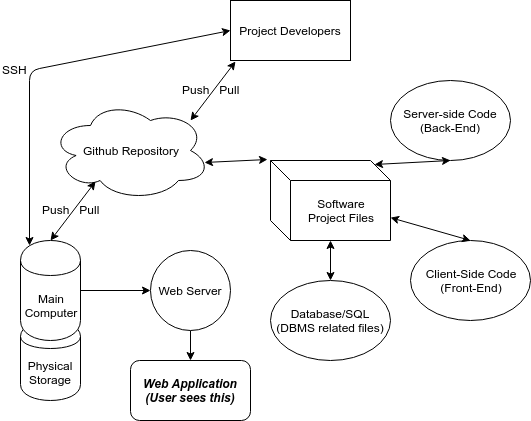
\includegraphics[ height=12cm]{ImplementationFigure} %width=xxcm
\end{center}

%*********************************************************************************************
%*********************************************************************************************
%
%				    Implementation
%
%*********************************************************************************************
%*********************************************************************************************
\pagebreak
\section*{Verification}
	The verification of the project will be performed by implementing different testing methods \cite {testmethod} with the web application. Firstly, unit testing will be implemented by testing individual aspects of the web application. For example, a customer is able to complete transaction to his or her request. So the implementation of unit testing here would exist as making sure each individual part of the transaction occurs correctly. In accordance to the ERD, the 'Invoice' is an entity with data that is updated atomically; specifically, this is the record of a transaction a customer may request. To unit test the entire transaction, code will be debugged with each iteration of the program until the transaction results in a feasible output (i.e. the invoice). By implementing unit testing during the development of the web application, each individual function of the web application will have higher success of functioning correctly because each function would have been tested to work individually.
	System testing is also a necessity for the project because system testing captures the users' perspectives and views, which is important in keeping integritive yet private data. System testing is best described as having a box with an input and output where specific users have specific views. In this project for example, if a customer orders a product, a customer would like to know what warehouse it is coming from but may not need to know who the supplier of the product is.
	Integration testing is the methodology of testing where developers test to see if their software works with different hardwares and interfaces. To actually have users of the application, users must be able to use their own devices and hardwares to access the application, which makes integral testing necesssary.
	Performance testing is a method of testing to see the efficiency of the application. For this project, performance testing will be implemented by having the product distribution service have relevant information readily available for different users.





%*********************************************************************************************
%*********************************************************************************************
%
%				     Verification
%
%*********************************************************************************************
%*********************************************************************************************
\pagebreak
\section*{Maintenance}  
	The maintenance of the project will be performed with various concepts to keep the deployed application stable. On a micro level, the development of the back-end (server side content) using JDBC will serve to maintain the integrity of the data as it is updated per user request. On the macro level, the maintenance of the project may consist of the project fixing bugs that users may find from interactions with the software, which would be refered to as patches. Additionally, maintenance includes the updating of present software's features with new features that make the user's experience easier or more efficient.




%*********************************************************************************************
%*********************************************************************************************
%
%				     Maintenance
%
%*********************************************************************************************
%*********************************************************************************************
\pagebreak
\begin{thebibliography}{9}
\bibitem{waterfall}
   \textit{Waterfall Model}\\
   \url{http://testingfreak.com/waterfall-model-software-testing-advantages-disadvantages-waterfall-model/}
\bibitem{testmethod}
   \textit{Testing Methodology}\\
   \url{https://www.guru99.com/testing-methodology.html}
\end{thebibliography}
  
\end{myspace}
\end{document}
